\documentclass{article}
\newcommand{\mydate}{December 10, 2025}
\newcommand{\mytitle}{QM HW10}
\title{\textbf{\mytitle}}
\author{Jiete XUE}
\date{\mydate}
\usepackage{fancyhdr}
\pagestyle{fancy}
\fancyhf{}
\fancyhead[C]{\mytitle }
\fancyhead[R]{Jiete Xue}
\fancyhead[L]{\mydate}
\fancyfoot[C]{\thepage}
\usepackage{amsthm}
\usepackage{amsmath}
\usepackage{amssymb}
\usepackage{bm}
\usepackage{enumitem}
\usepackage{physics}
\usepackage{tikz}
\usetikzlibrary{arrows.meta, decorations.markings}
\usepackage{float}

%% 右矢
%\ket{\psi}          % 输出:|ψ⟩
%\ket{\psi(t)}       % 输出:|ψ(t)⟩
%
%% 左矢
%\bra{\phi}          % 输出:⟨φ|
%
%% 期望值
%\expval{\hat{A}}    % 输出:⟨Â⟩
%\expval{\hat{A}}{\psi}  % 输出:⟨ψ|Â|ψ⟩
%
%% 对易子
%\comm{\hat{A}}{\hat{B}}  % 输出:[Â, B̂]
\newtheoremstyle{1}{}{}{}{}{\bfseries}{}{\newline}{}
\theoremstyle{1}
\newtheorem{problem}{Problem}
\newtheorem{solution}{Solution}
\usepackage{chngcntr}
\counterwithin{equation}{problem}

\setlist[enumerate]{label=(\arabic*), leftmargin=*, align=left}

\newcommand{\pa}{\partial}
\newcommand{\rn}[1]{\romannumeral #1\relax}
\newcommand{\Rn}[1]{\expandafter\@slowromancap\romannumeral#1@}
\newcommand{\ii}{\mathrm{i}}
\newcommand{\ee}{\mathrm{e}}

\begin{document}
\maketitle
\begin{problem}
\begin{equation}
    H'(t)=-\frac{F_0 \tau /\omega}{\tau^2+t^2} x = -\frac{F_0 \tau /\omega}{\tau^2+t^2} \frac{a+a^\dagger}{\sqrt{2}}\sqrt{\frac{\hbar}{m\omega}}.
\end{equation}
\begin{equation}
    c^{(1)}=\frac{-\ii}{\hbar}\int_{-\infty}^{+\infty}\dd{t} \exp(\ii \omega t)\bra{1}H'\ket{0}=\frac{\ii F_0}{\sqrt{2\hbar m \omega^3}}\int_{-\infty}^{+\infty}\ee^{\ii \omega \tau z}\frac{\dd z}{1+z^2}.
\end{equation}

\begin{center}
    

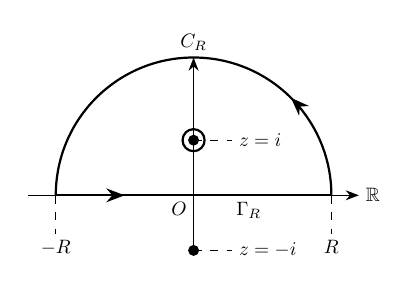
\begin{tikzpicture}[
    >=Stealth,
    contour/.style={thick, decoration={markings, mark=at position 0.25 with {\arrow{>}}}, postaction={decorate}},
    axis/.style={->},
    pole/.style={fill=black, circle, inner sep=2pt},
    dim/.style={dashed},
    scale=0.7,
    transform shape
]

% 坐标轴
\draw[axis] (-3,0) -- (3,0) node[right] {$\mathbb{R}$};
\draw[axis] (0,-1) -- (0,2.5) node[above] {};

% 实轴部分(围道的一部分)
\draw[contour] (-2.5,0) -- node[below, pos=0.7] {$\Gamma_R$} (2.5,0);
% 上半圆弧(半径 R,逆时针)
\draw[contour] (2.5,0) arc (0:180:2.5) node[midway, above] {$C_R$};

% 奇点(极点)
\node[pole, label=left:{}] at (0,1) {};
\node[pole, label=right:{}] at (0,-1) {};

% 用虚线标出 -R 和 R
\draw[dim] (-2.5,0) -- (-2.5,-0.7) node[below] {$-R$};
\draw[dim] (2.5,0) -- (2.5,-0.7) node[below] {$R$};

% 虚轴虚线
\draw[dim] (0,-1) -- (0,2.2);
% 极点标记
\draw[dim] (0,1) -- (0.7,1) node[right] {$z = i$};
\draw[dim] (0,-1) -- (0.7,-1) node[right] {$ z = -i$};

% 箭头指示绕行方向
\node at (1.8,1.2) {};

% 图示说明:只有上半平面的极点被包围
\draw[thick] (0,1) circle (0.2);
\node[right] at (0.4,1.2) {};

% 原点标记
\node at (0,0) [below left] {$O$};

\end{tikzpicture}
\end{center}
By residue theorem,
\begin{equation}
    \int_{-\infty}^{+\infty}\ee^{\ii \omega \tau z}\frac{\dd z}{1+z^2}=\pi \ee^{-\omega \tau}.
\end{equation}
So, 
\begin{equation}
    P = |c^{(1)}|^2=\frac{\pi^2 F_0^2 \ee^{-2\omega \tau}}{2\hbar m\omega ^3}.
\end{equation}
$\tau\gg 1/\omega$ means low frequency of transition, it is proper.
\end{problem}
\begin{problem}
    \begin{equation}
        H'(t)=e E_0 z \exp(-t/\tau),\ t>0.
    \end{equation}
    \begin{equation}
        c^{(1)}_f(+\infty)=\frac{-\ii }{\hbar}\int_{0}^{+\infty} \dd{t}' \bra{f}H'(t)\ket{i}\ee^{\ii \omega_{fi} t'}.
    \end{equation}
    \begin{equation}
        \bra{f}z\ket{i}=\sqrt{\frac{4\pi}{3}}\bra{R_{nl}}r\ket{R_{10}}\cdot\bra{Y_l^m} Y_1^0 \ket{Y_0^0}.
    \end{equation}
    Since $Y_1^0$ is odd and by Wigner-Eckart theorem, only $l=1$ and $m=0$, the element can not be zero.
    \begin{equation}
        \bra{Y_l^m} Y_1^0 \ket{Y_0^0}=\frac{1}{\sqrt{4\pi}} \int |Y_1^0|^2\dd{\Omega}=\frac{1}{\sqrt{4\pi}}.
    \end{equation}
    \begin{equation}
        \int_{0}^{+\infty}\ee^{-t/\tau+\ii \omega_{fi}t}\dd t= \frac{1}{1/\tau -\ii \omega_{fi}}.
    \end{equation}
    So,
    \begin{equation}
        P_{210}= \frac{e^2 E_0^2 |\bra{R_{nl}}r\ket{R_{10}}|^2 \tau^2}{2 \hbar^2 \left(1+ \omega^2 \tau^2\right)}.
    \end{equation}
    where $E_0$ is the energy of ground state, and $\omega=\frac{3}{4}\frac{E_0}{\hbar}$.
\end{problem}
\begin{problem}
(a) 
Let 
\begin{equation}
    \Delta \omega = \omega - \omega_{21}.
\end{equation}
Define new variables:
\begin{equation}
    \tilde{c}_1(t) = c_1(t) e^{-i\Delta\omega\, t/2}, \qquad
    \tilde{c}_2(t) = c_2(t) e^{i\Delta\omega\, t/2}.
\end{equation}
Then,
\begin{equation}
    i\hbar \dv{}{t}
    \begin{pmatrix}
    \tilde{c}_1 \\ \tilde{c}_2
    \end{pmatrix}
    =
    \frac{\hbar}{2}
    \begin{pmatrix}
    \Delta\omega & 2\gamma/\hbar \\[4pt]
    2\gamma/\hbar & -\Delta\omega
    \end{pmatrix}
    \begin{pmatrix}
    \tilde{c}_1 \\ \tilde{c}_2
    \end{pmatrix}.
\end{equation}

Thus the effective Hamiltonian in the rotated frame is

\begin{equation}
    H_{\text{eff}} = \frac{\hbar}{2}
    \begin{pmatrix}
    \Delta\omega & 2\gamma/\hbar \\[4pt]
    2\gamma/\hbar & -\Delta\omega
    \end{pmatrix}
    = \frac{\hbar}{2}\Bigl( \Delta\omega\,\sigma_z + \frac{2\gamma}{\hbar}\,\sigma_x \Bigr).
\end{equation}
\begin{equation}
    U(t) = \exp\!\Bigl( -\frac{i}{\hbar} H_{\text{eff}} \, t \Bigr)
          = \exp\!\Bigl[ -i t 
            \begin{pmatrix}
              \Delta\omega/2 & \gamma/\hbar \\[4pt]
              \gamma/\hbar   & -\Delta\omega/2
            \end{pmatrix}
            \Bigr].
\end{equation}

The eigenvalues of the matrix are \(\pm \Omega_R\) with

\begin{equation}
    \Omega_R = \sqrt{ \Bigl(\frac{\gamma}{\hbar}\Bigr)^2 + \Bigl(\frac{\Delta\omega}{2}\Bigr)^2 }.
\end{equation}

Using the identity \(\exp(-i \bm{n}\cdot\bm{\sigma}\,\theta) = \cos\theta\, I - i\sin\theta\, (\bm{n}\cdot\bm{\sigma})\), we obtain

\begin{equation}\label{3.7}
    U(t) = \cos(\Omega_R t) \, I
          - i \sin(\Omega_R t) \,
            \frac{1}{\Omega_R}
            \begin{pmatrix}
              \Delta\omega/2 & \gamma/\hbar \\[4pt]
              \gamma/\hbar   & -\Delta\omega/2
            \end{pmatrix}.
\end{equation}

With \(\tilde{c}_1(0)=1,\ \tilde{c}_2(0)=0\), equation \eqref{3.7} gives

\begin{equation}
    \tilde{c}_2(t) = -i\,\frac{\gamma}{\hbar\Omega_R} \sin(\Omega_R t).
\end{equation}


Returning to the original variables,

\begin{equation}
    c_2(t) = \tilde{c}_2(t) e^{-i\Delta\omega\, t/2}
           = -i\,\frac{\gamma}{\hbar\Omega_R} e^{-i\Delta\omega\, t/2} \sin(\Omega_R t).
\end{equation}

Hence the occupation probability of the excited state is

\begin{equation}
    \boxed{\;
    |c_2(t)|^2 = \frac{\gamma^2/\hbar^2}{\gamma^2/\hbar^2 + (\omega-\omega_{21})^2/4} 
                 \sin^2\!\Bigl[ \sqrt{ \frac{\gamma^2}{\hbar^2} + \frac{(\omega-\omega_{21})^2}{4} } \; t \Bigr]
    \;}
\end{equation}
and, by normalization,

\begin{equation}
    |c_1(t)|^2 = 1 - |c_2(t)|^2.
\end{equation}
(b) 
\begin{equation}
    c_2^{(1)}(t)= -\frac{\ii }{\hbar} \gamma \int_{0}^{t}\ee^{-\ii \Delta \omega t'} \dd{t'}=\frac{\gamma}{\hbar \Delta \omega}(1-\ee^{-\ii \Delta t}).
\end{equation}
So,
\begin{equation}
    P_{1\rightarrow 2}^{(1)}(t)=\frac{4\gamma^2}{\hbar^2 \Delta \omega^2}\sin^2\left(\frac{\Delta \omega t}{2}\right).
\end{equation}
For the cases where $\Delta \omega \gg \frac{\gamma}{\hbar}$, the approximation is valid. But for the cases where $\Delta \omega \ll \frac{\gamma}{\hbar}$, the approximation is not valid. This is because this resonance case.
\end{problem}
\begin{problem}
    \begin{equation}
        H'(t)=e E_0 (x\cos(\omega t)-y\sin(\omega t)),\ t>0.
    \end{equation}
    \begin{equation}
        x\cos(\omega t)-y\sin(\omega t)\sim (Y_1^{+1}+Y_1^{-1})\cos(\omega t) + \ii (Y_1^{+1}-Y_1^{-1})\sin(\omega t).
    \end{equation}
    That is 
    \begin{equation}
        H'(t)\sim Y_1^{+1} \ee^{\ii \omega t} + Y_1^{-1} \ee^{-\ii \omega t}.
    \end{equation}
    Since $x$, $y$ has odd parity and by Wigner-Eckart theorem, only when $\Delta m=\pm 1$, $\Delta l=\pm 1$, the element can not be zero.
\end{problem}
\begin{problem}
    (a) We have shown that the possible final states should be $l'=1$ and $m'=0/\pm 1$. By symmetry, three banch have the same ratio.
    \newline
    (b) $l'=l\pm 1$, $m'= m \text{ or } m \pm 1$. By Wigner-Eckart theorem,
    \begin{equation}
        P(m')= |\braket{l,m;1,(m'-m)}{l',m'}|^2
    \end{equation}
    (1) For a fixed $l'$, the ratio is 
    \begin{equation}
        |\braket{l,m;1,-1}{l',m-1}|^2 : |\braket{l,m;1,0}{l',m}|^2 : |\braket{l,m;1,1}{l',m+1}|^2.
    \end{equation}
    (2) 
\end{problem}
\end{document}



